\documentclass[11pt]{article}
\pdfinfoomitdate=1
\pdftrailerid{}
\pdfsuppressptexinfo=15
\usepackage[T1]{fontenc}
\usepackage{mathpazo}
\usepackage[margin=1in]{geometry}
\usepackage{amsmath,amssymb,amsthm,mathtools}
\usepackage{mathrsfs}
\usepackage{microtype}
\usepackage{xcolor}
\usepackage{tikz}
\usepackage[colorlinks=true,linkcolor=blue!45!black,citecolor=blue!45!black,urlcolor=blue!45!black]{hyperref}
\hypersetup{pdftitle={Taming implies compatibility on four-manifolds},pdfauthor={OpenAI},pdfsubject={Donaldson's tamed-to-compatible conjecture}}
\newtheorem{theorem}{Theorem}[section]
\newtheorem{proposition}[theorem]{Proposition}
\newtheorem{lemma}[theorem]{Lemma}
\newtheorem{corollary}[theorem]{Corollary}
\theoremstyle{remark}
\newtheorem{remark}[theorem]{Remark}
\newtheorem{example}[theorem]{Example}
\numberwithin{equation}{section}
\newcommand{\R}{\mathbb R}
\newcommand{\vol}{\,dV_g}
\newcommand{\dd}{\,d}
\newcommand{\im}{\operatorname{im}}
\newcommand{\supp}{\operatorname{supp}}
\newcommand{\pr}{\operatorname{pr}}
\newcommand{\Id}{\mathrm{id}}
\newcommand{\ind}{\mathbf 1}
\newcommand{\norm}[1]{\left\lVert #1\right\rVert}
\newcommand{\abs}[1]{\left\lvert #1\right\rvert}
\newcommand{\ip}[2]{\left\langle #1,#2\right\rangle}
\newcommand{\cL}{\mathcal L}
\newcommand{\ang}{\mathcal I}
\newcommand{\trans}{\mathcal N}
\newcommand{\eps}{\varepsilon}
\setlength{\emergencystretch}{2em}
\urlstyle{same}
\makeatletter
\renewcommand{\@maketitle}{%
  \newpage
  \null
  \vskip 2em
  \begin{center}
    {\LARGE \@title \par}
    \vskip 0.8em
    {\large \@author \par}
    \vskip 0.5em
    {\@date \par}
  \end{center}
  \par
  \vskip 1em
}
\makeatother

\title{Taming implies compatibility on four-manifolds}
\author{OpenAI}
\date{October 6, 2026}
\begin{document}
\maketitle
\begin{abstract}
We prove that every smooth almost complex structure on a closed four-manifold
which is tamed by a symplectic form is compatible with a symplectic form.
This gives a positive solution to Donaldson's tamed-to-compatible conjecture.
We also characterize the compatible cone by strict intersection positivity
on the closure of the invariant part of the taming cone.
\end{abstract}
\section{Introduction}

Let \(X\) be a closed smooth four-manifold and let \(J\) be a smooth
almost complex structure on \(X\). A smooth real two-form \(\omega\)
is symplectic if it is nondegenerate and closed, meaning
\(d\omega=0\). A real two-form \(\omega\)
\emph{tames} \(J\) if \(\omega(v,Jv)>0\) for every nonzero tangent
vector \(v\). It is \emph{compatible} with \(J\) if, in addition,
\(\omega(Ju,Jv)=\omega(u,v)\). A taming form is automatically
nondegenerate; thus a closed taming form is symplectic.

Donaldson asked whether the existence of a taming symplectic form
on a closed four-manifold implies the existence of a compatible
one \cite[Section~5.2, Question~2]{Donaldson2006}.
This existence question is distinct from his a priori estimate
conjecture for a prescribed-volume equation.
The elementary projection
\(\omega\mapsto \frac12(\omega+\omega(J\,\cdot,J\,\cdot))\)
shows the obstacle: it preserves positivity on complex lines
but generally loses closedness. Our main result answers the
existence question affirmatively.

\begin{theorem}\label{thm:main}
Suppose that a smooth almost complex structure \(J\) on a closed
connected smooth real four-manifold \(X\) is tamed by a symplectic
form. Then there is a smooth symplectic form compatible with \(J\).
\end{theorem}

The almost complex structure in Theorem~\ref{thm:main} is the given
one. The conclusion imposes no condition on the cohomology class of
the compatible form. In particular, it does not assert that an
arbitrary taming class contains a compatible representative.

There is also an intrinsic description of the compatible cone in terms
of the taming cone and the intersection pairing.

\begin{theorem}[Taming and compatible cones]\label{thm:taming-cones}
Let \(X,J\) satisfy the hypotheses of Theorem~\ref{thm:main}, and give
\(X\) the orientation induced by \(J\). Let
\(\mathcal K_J^t,\mathcal K_J^c\subset H^2(X;\R)\) be the classes
represented by taming and compatible symplectic forms, respectively.
Let \(H_J^-\) be the subspace represented by smooth closed real
anti-invariant two-forms. Set
\[
 \mathcal V=(H_J^-)^\perp,\qquad
 \mathcal C=\mathcal K_J^t\cap\mathcal V,
\]
where orthogonality is for the intersection pairing. Then
\begin{align}
 \mathcal K_J^t&=\mathcal C+H_J^-,\label{eq:tame-decomposition}\\
 \mathcal K_J^c&=
 \{a\in\mathcal C:\ a\cdot y>0
   \text{ for every }0\ne y\in\overline{\mathcal C}\}.
 \label{eq:compatible-duality}
\end{align}
The closure is taken in \(\mathcal V\), and the sum in
\eqref{eq:tame-decomposition} is a Minkowski sum.
\end{theorem}

\begin{corollary}\label{cor:taming-cones}
Under the same hypotheses, write \(h_J^-=\dim H_J^-\) and let
\(b_2^+(X)\) be the positive index of the intersection form.
If \(h_J^-=b_2^+(X)-1\), then
\[
 \mathcal K_J^t=\mathcal K_J^c+H_J^-.
\]
In particular, if \(b_2^+(X)=1\), then
\(\mathcal K_J^t=\mathcal K_J^c\): every taming class has a smooth
compatible symplectic representative.
\end{corollary}

The proofs are given in Section~\ref{sec:cones}. They use separation
in a prescribed cohomology class and the current estimates below.
The inclusion
\(\mathcal K_J^c+H_J^-\subseteq\mathcal K_J^t\)
can be strict when \(h_J^-<b_2^+-1\), even if \(H_J^-=0\);
Example~\ref{ex:strict-cones} gives an explicit four-torus.

The integrable case belongs to the theory of compact complex surfaces.
Buchdahl \cite[Theorem~11]{Buchdahl1999} and Lamari
\cite[Corollary~5.7]{Lamari1999} gave classification-free proofs
that even first Betti number implies the existence of a K\"ahler metric.
Lamari's positive exact current on a surface with odd first Betti number
also obstructs a taming form \cite[Theorem~6.1]{Lamari1999}.
Li and Zhang proved the equivalence between the existence of taming
and compatible symplectic forms on complex surfaces
\cite[Theorem~1.2]{LiZhang2009}.

The pseudoholomorphic-curve approach has a different starting point.
For structures on \(\mathbb{CP}^2\) tamed by the standard symplectic
form, Gromov constructed a compatible form by averaging currents
of pseudoholomorphic lines \cite[Section~2.4.A$'$]{Gromov1985}.
Taubes developed integration over curve moduli spaces to obtain
compatibility for a residual subset of the smooth almost complex
structures tamed by a fixed symplectic form when \(b_2^+=1\)
\cite{Taubes2011,Taubes2017}.
Theorem~1 of \cite{Taubes2011} also states preservation of the taming
form's cohomology class when that class is rational.
Li and Zhang extended this approach to every tamed structure on
\(S^2\times S^2\) and
\(\mathbb{CP}^2\#\overline{\mathbb{CP}}{}^2\), and to further
rational manifolds under hypotheses on embedded pseudoholomorphic
spheres \cite[Theorems~1.2 and~1.3]{LiZhang2015}.

An invariant two-form satisfies
\(\alpha(Ju,Jv)=\alpha(u,v)\); an anti-invariant one satisfies
\(\alpha(Ju,Jv)=-\alpha(u,v)\).
Write \(h_J^-=\dim H_J^-\), where \(H_J^-\) is the anti-invariant
cohomology space defined in Theorem~\ref{thm:taming-cones}.
The condition \(h_J^-=b_2^+-1\) occurs in Buchdahl-type approaches
\cite{TWZZ2022,LinZhou2025}, in the compatibility criteria of
Wang, Wang and Zhu \cite[Theorems~4.3 and~5.1]{WangWangZhu2023},
and in the taming corollary of Wang, Zhang, Zheng and Zhu
\cite[Corollary~1.3]{WangZhangZhengZhu2025}.
The latter paper's generalized Monge--Amp\`ere theorem starts with
an almost K\"ahler structure.
Li and Ning's recent study of spaces of K\"ahler and holomorphically
tamed forms allows the integrable complex structure to vary
\cite{LiNing2026}.

The current approach has a classical cone-duality background.
Sullivan related closed forms positive on a field of tangent directions
to the corresponding structure currents \cite{Sullivan1976}.
Harvey and Lawson characterized K\"ahler manifolds through positive
currents \cite{HarveyLawson1983}; Li and Zhang developed the
almost-complex formulation used to compare taming and compatibility
\cite[Section~3]{LiZhang2009}.
In the argument below, separation gives a positive functional vanishing
on closed invariant forms. An explicit elliptic lift and quantitative
current estimates connect this obstruction to the existence
of a taming form.

\subsection*{The argument and its main estimate}

Fix an auxiliary \(J\)-Hermitian metric. If no compatible form
exists, separation produces a nonzero positive current \(P\)
that annihilates closed invariant forms. An elliptic correction
gives \(T=P+Q\), which annihilates every closed two-form, with
\(Q\) initially an anti-invariant distribution. Represent \(P\)
as a positive weighted average of unit complex-line bivectors,
and let \(\mu\) be the resulting measure on \(X\), its trace measure.
Corrected radial test functions give \(\mu(B_r(x))\le Cr^2\).
Regularization by a finite power of the Hodge resolvent then
proves \(Q\in L^2\) and an angular estimate: over pairs of
complex lines in this representation whose base points are
less than \(r\) apart, the integral of their squared difference,
after parallel transport, is \(O(r^4)\).

The first regularized pairing only bounds \(\|Q\|_2\), because
the negative error in this pairing is only uniformly bounded.
To remove that error, we distinguish the points where \(P\)
has positive two-dimensional density. Write
\[
\theta(x)=\lim_{r\downarrow0}r^{-2}\mu(B_r(x)),
\qquad E=\{x:\theta(x)>0\}.
\]
Existence of the limit is part of the argument. The principal
step, Theorem~\ref{thm:splitting}, proves that the restriction
\(P_E=\ind_E P\) is closed. It applies to any closed current
\(P+Q\) with an anti-invariant \(L^2\) correction and the stated
mass and angular bounds; annihilation of all closed forms is
not needed for this step.

The reason the angular estimate suffices is a balance between
two errors. Planar tangent measures show that, over the same
nearby pairs, the squared normal component of the displacement
between base points, relative to the first complex line and divided
by \(r^2\), has integral \(o(r^2)\).
Closedness of \(P+Q\) trades tangential derivatives of a smooth
density cutoff for a product of angular and transverse errors.
The derivative and normalization of the cutoff contribute
\(r^{-3}\). Cauchy--Schwarz therefore bounds the decisive
boundary term by
\[
r^{-3}\,O(r^2)\,o(r)=o(1),
\]
where the two factors are the square roots of the angular and
transverse moments. The \(L^2\) bound controls the correction's
cutoff error separately. Together these estimates prove closedness
of the density restriction without requiring a quantitative rate
for tangent measure convergence.

Once \(P_E\) is closed, the residual
\(T-P_E=\ind_{X\setminus E}P+Q\) is closed as well. Its positive
summand is concentrated on zero-density centers, where the
negative error in the pairing does tend to zero. Pairing this residual
with \(T\), and using the vanishing of the mixed terms, forces
\(Q=0\). The resulting nonzero positive current \(P=T\)
cannot annihilate a closed taming form.

The relative projection estimate in Lemma~\ref{lem:mixing}, for
fixed smooth orthogonal bundle projections, and the closedness
statement in Theorem~\ref{thm:splitting} may be useful separately.
The regularized pairing estimates use the four-dimensional fact
that anti-invariant two-forms are self-dual.
Sections~\ref{sec:currents} and \ref{sec:mass} construct the
separating current and prove its mass bound.
Section~\ref{sec:energy} establishes the regularization and
angular estimates. Section~\ref{sec:density} proves density
existence and the planar tangent description;
Section~\ref{sec:splitting} uses them to control cutoff boundaries
and prove closedness of \(P_E\).
Section~\ref{sec:conclusion} completes the existence argument.
Section~\ref{sec:cones} develops the prescribed-class separation
and proves the cone description.

A triple of closed two-forms on an oriented four-manifold is
\emph{hypersymplectic} if every nonzero real linear combination is
symplectic and induces the given orientation. The companion
\cite[Theorem~1.1]{OpenAIHypersymplectic2026} combines the current
estimates above with additional prescribed-class and deformation
arguments to deform hypersymplectic triples normalized by
\(\int_X\omega_i\wedge\omega_j=\delta_{ij}\) on closed connected oriented
smooth four-manifolds to hyperk\"ahler triples, while fixing each class
\([\omega_i]\in H^2(X;\R)\).

\section{A current obtained by separation}\label{sec:currents}

We first construct the current that would obstruct compatibility:
a positive current and an anti-invariant correction whose sum
annihilates every closed two-form.

Give \(X\) its complex orientation. Fix a smooth \(J\)-Hermitian
metric \(g\), and write
\[
F(u,v)=g(Ju,v),\qquad
(R\alpha)(u,v)=\tfrac12\bigl(\alpha(u,v)-\alpha(Ju,Jv)\bigr).
\]
Thus \(R\) is the orthogonal projection onto the anti-invariant
two-forms, and \(1-R\) projects onto the invariant two-forms.
All forms and currents are real.

We identify bivectors with two-forms using \(g\). Let
\(\mathscr C\to X\) be the bundle of unit complex line bivectors
\[
\mathscr C_x=\{v\wedge Jv:\ |v|_g=1\}.
\]
For \(\ell\in\mathscr C_x\), let \(L_\ell\subset T_xX\) be its
oriented plane. The following pointwise identities will be used:
\begin{equation}\label{eq:algebra}
\im R\subset\Lambda_g^+,\qquad
*F=F,\qquad |F|^2=2,\qquad
|\ell|=1,\qquad \ell^+=F/2,\qquad F(\ell)=1.
\end{equation}
They follow by taking a unitary frame
\((v,Jv,w,Jw)\). In that frame \(F\) corresponds to
\(v\wedge Jv+w\wedge Jw\), and the anti-invariant subspace is spanned
by
\[
v\wedge w-Jv\wedge Jw,\qquad
Jv\wedge w+v\wedge Jw.
\]

A two-current acts on smooth two-forms. It is \emph{closed} if it
annihilates exact two-forms. Under the \(L^2\) identification with
distributional two-forms, this means \(d^*T=0\), or equivalently
\(d(*T)=0\). Multiplication and orthogonal projections on
distributional forms act on currents by duality.

\begin{lemma}[A closed lift]\label{lem:lift}
There is a real order-zero pseudodifferential operator
\[
B:C^\infty(\im R)\longrightarrow\Omega^2(X)
\]
such that \(dB=0\) and \(RB=\Id\).
\end{lemma}

\begin{proof}
Consider \(\cL=Rdd^*\) on sections of \(\im R\). If \(\xi\ne0\),
the projection of
\(\xi\wedge\iota_{\xi^\sharp}\) from self-dual two-forms back to
self-dual two-forms is \(|\xi|^2/2\) times the identity.
By \eqref{eq:algebra}, the principal symbol of \(\cL\) on
\(\im R\) is therefore the same scalar. In particular \(\cL\)
is elliptic. For anti-invariant smooth forms \(a,b\),
\[
\ip{\cL a}{b}_{L^2}=\ip{d^*a}{d^*b}_{L^2}.
\]
It is nonnegative and self-adjoint. Every element of its kernel
is smooth and coclosed; being self-dual, it is also closed.

Let \(H\) be the orthogonal projection onto this kernel and let
\(G\) be the inverse of \(\cL\) on its orthogonal complement,
extended by zero on the kernel. The elliptic generalized-inverse
theorem gives \(G\) of order \(-2\) and \(H\) a smoothing
finite-rank operator; see
\cite[Proposition~6.4 and Theorem~6.3]{MelroseIML}.
Set
\[
B=dd^*G+H.
\]
Then \(dB=0\), while \(RB=\cL G+H=\Id\).
\end{proof}

The projected elliptic operator used here also appears in Lejmi's
proof of local compatibility in dimension four
\cite[proof of Theorem~1]{Lejmi2006}.
Dr\u{a}ghici and Zhang's exact-form result gives the corresponding
global linear correction phenomenon
\cite[Proposition~3.1]{DraghiciZhang2012}.
The present formula specifies the closed lift and its mapping properties;
positivity remains a separate problem.

\begin{proposition}\label{prop:separation}
If \(J\) admits no compatible symplectic form, there are currents
\(P,Q,T\) and a finite positive measure \(\lambda\) on
\(\mathscr C\) such that
\begin{align}
P(\alpha)&=\int_{\mathscr C}\alpha_x(\ell)\dd\lambda(x,\ell),
&\lambda(\mathscr C)&=1,\label{eq:positive-representation}\\
T&=P+Q,
&RP&=0,\quad RQ=Q,\quad *Q=Q,\label{eq:decomposition}\\
T(\alpha)&=0&&\text{for every smooth closed two-form }\alpha.
\label{eq:annihilation}
\end{align}
The current \(P\) annihilates every closed invariant two-form.
The projection \(\mu\) of \(\lambda\) to \(X\) is the
\emph{trace measure} of \(P\): for every smooth function \(b\),
\(P(bF)=\int_Xb\dd\mu\). Each of \(P,Q,T\) belongs to \(H^{-3}\).
\end{proposition}

\begin{proof}
In the Fr\'echet space of smooth invariant two-forms, the cone of
positive definite forms is open and convex. It is disjoint from
the linear subspace of closed invariant forms by hypothesis.
Hahn--Banach separation gives a nonzero continuous functional
nonnegative on the cone and zero on that subspace. Extend it to
all two-forms by composing with \(1-R\), and call it \(P\).
This is the positive-current separation framework of
Sullivan and Harvey--Lawson \cite{Sullivan1976,HarveyLawson1983};
for its almost-complex formulation, see
\cite[Section~3]{LiZhang2009}.

Positivity extends to semidefinite invariant forms by adding
\(\eps F\) and taking \(\eps\downarrow0\).
Since \(C\|\alpha\|_\infty F\pm(1-R)\alpha\) are semidefinite
for a fixed norm-comparison constant,
\[
|P(\alpha)|\le C\|\alpha\|_\infty P(F).
\]
Thus \(P\) has order zero, and \(P(F)>0\) because \(P\ne0\).
Scale \(P\) so that \(P(F)=1\).

For completeness, the measure representation can be obtained
in local unitary frames. Invariant two-forms identify with
Hermitian symmetric forms by
\(\alpha\mapsto\alpha(\,\cdot,J\,\cdot)\).
The positive functional has a positive Hermitian matrix of
coefficient measures. Its trace is a positive measure \(\mu\);
the coefficient measures are absolutely continuous with
respect to \(\mu\). Their Radon--Nikodym density is a positive
semidefinite Hermitian matrix of trace one, or equivalently
a convex combination of bivectors in \(\mathscr C_x\).
Measurable spectral decomposition in measurable unitary frames
gives \(\lambda\) in \eqref{eq:positive-representation}.
The identity \(F(\ell)=1\) shows that its projection is \(\mu\)
and that its total mass is one.

Define
\[
T(\alpha)=P(\alpha-BR\alpha),\qquad
Q(\alpha)=-P(BR\alpha).
\]
For closed \(\alpha\), the form \(\alpha-BR\alpha\) is closed
and invariant, proving \eqref{eq:annihilation}. Moreover \(RP=0\)
and \(RQ=Q\), so \(*Q=Q\) by \eqref{eq:algebra}.
In particular \(T\) is a closed current.

A finite measure on a compact four-manifold defines an element
of \(H^{-3}\), by the Sobolev embedding \(H^3\subset C^0\).
The order-zero operator \(RB^*\) is bounded on this Sobolev
space by the pseudodifferential Sobolev mapping theorem
\cite[Proposition~0.5.E]{Taylor1991}, so the same conclusion
holds for \(Q=-RB^*P\) and \(T\).
\end{proof}

Hereafter \(C\), with or without a subscript, denotes a finite
constant independent of the small scale parameters. It may
change from one occurrence to the next. Constants are uniform
over centers in \(X\).

\section{Quadratic mass growth}\label{sec:mass}

Let \(P,\mu\) be as in Proposition~\ref{prop:separation}.
We use the annihilation of closed invariant forms to bound the
mass of \(P\) in every small ball.
Write \(B_s(x)\) for a geodesic ball.
\begin{proposition}\label{prop:growth}
There is a constant \(C\) such that
\begin{equation}\label{eq:growth}
\mu(B_s(x))\le Cs^2
\end{equation}
for all \(x\in X\) and \(s>0\).
\end{proposition}

The proof uses closed invariant test forms
\[
Du=(1-BR)dd_J^cu,\qquad d_J^cu=-du\circ J.
\]
The Hessian terms of \(dd_J^cu\), with \(J\) frozen at a point,
form an invariant two-form. Consequently \(Rdd_J^c\) is a
first-order differential operator on functions.

We first spell out the local estimate needed for the
order-zero correction. In dimension four, an order-zero
pseudodifferential operator has an off-diagonal kernel bounded
by \(C|y-z|^{-4}\) in local coordinates
\cite[Section~0.2, Proposition~0.2.B]{Taylor1991}.
Work in a fixed smooth local bundle trivialization.
If \(f\) is supported in a coordinate ball of radius \(a\le1\)
and its coefficient derivatives satisfy
\begin{equation}\label{eq:scaled-input}
|\partial^jf|\le C_jMa^{-j},
\end{equation}
then its local contribution to the operator is bounded by
\(CM\). Indeed, write \(f(z)=M\widetilde f((z-z_0)/a)\).
Six bounded derivatives of \(\widetilde f\) give
\(|\widehat{\widetilde f}(\xi)|\le C(1+|\xi|^2)^{-3}\)
by integration by parts. This bound is integrable in four
dimensions, so \(\|\widehat{\widetilde f}\|_1\le C\), and hence
\(\|\widehat f\|_1\le CM\). The bounded-symbol Fourier formula
gives the assertion; smoothing remainders are controlled by
\(\|f\|_1\). This estimate uses the derivative bounds
\eqref{eq:scaled-input}, not general \(L^\infty\) boundedness.

\begin{lemma}\label{lem:radial-correction}
Choose normal coordinates centered at \(x\), on a uniformly
small fixed ball, and put \(t=d_g(x,y)\). Let a smooth radial
cutoff be one on a smaller ball and vanish outside the
coordinate ball. For \(s>0\) small, let \(u_s,h_s\) be this
cutoff times
\[
\log\sqrt{s^2+t^2},\qquad \sqrt{s^2+t^2},
\]
respectively, extended by zero. Near the center,
\begin{equation}\label{eq:correction-bounds}
|BRdd_J^cu_s|\le \frac{C}{s+t},
\qquad
|BRdd_J^ch_s|\le C(1+|\log(s+t)|).
\end{equation}
Both expressions are uniformly bounded at any fixed positive
distance from \(x\).
\end{lemma}

\begin{proof}
The first-order property of \(Rdd_J^c\) gives
\[
|\partial^j(Rdd_J^cu_s)|\le C_j(s+t)^{-1-j},\qquad
|\partial^j(Rdd_J^ch_s)|\le C_j(s+t)^{-j}
\]
near \(x\). Away from \(x\), all fixed-order derivatives are
uniformly bounded, including terms from the cutoff.

At \(y\), put \(a=s+t\), assuming \(a\) small. Localize the
input to a ball about \(y\) of radius a small fixed multiple
of \(a\). On this ball \(s+d_g(x,\cdot)\) is comparable to
\(a\), so \eqref{eq:scaled-input} gives contributions \(C/a\)
and \(C\). For the rest of the input within distance \(O(a)\)
of \(x\), the kernel is bounded by \(Ca^{-4}\). The respective
input \(L^1\) bounds on this region are \(Ca^3\) and \(Ca^4\),
again giving \(C/a\) and \(C\).

On the more distant shells about \(x\), with radius
\(\rho\ge Ca\), the kernel is \(O(\rho^{-4})\), the input
bounds are \(C/\rho\) and \(C\), and the shell volume is
\(O(\rho^4)\). Summation over dyadic shells gives \(C/a\)
and \(C(1+|\log a|)\). The logarithmic input has uniformly
bounded total \(L^1\) norm, since its local integral is at most
\(C\int_0^{\rho_0}\rho^3/(s+\rho)\dd\rho\le C\rho_0^3\).
The square-root input has bounded \(L^1\) norm as well.
Thus the remaining smooth kernel terms are bounded uniformly.
The same decomposition gives uniform bounds
when \(y\) stays a fixed distance from the center.
Compactness makes all chart and operator constants uniform
in \(x\).
\end{proof}

\begin{proof}[Proof of Proposition~\ref{prop:growth}]
In the normal coordinates of Lemma~\ref{lem:radial-correction},
let \(J_0=J(x)\) be the constant complex structure, orthogonal
for the Euclidean metric at the center. On the inner ball,
the Hessians of the two radial functions are
\[
\frac{I}{s^2+t^2}-\frac{2zz^\top}{(s^2+t^2)^2},
\qquad
\frac{I}{\sqrt{s^2+t^2}}-\frac{zz^\top}{(s^2+t^2)^{3/2}}.
\]
Since
\((z\cdot v)^2+(z\cdot J_0v)^2\le t^2|v|^2\), their
complex-line traces satisfy
\begin{align}
dd^c_{J_0}u_s(v,J_0v)
&\ge\frac{2s^2|v|^2}{(s^2+t^2)^2},\label{eq:log-trace}\\
dd^c_{J_0}h_s(v,J_0v)
&\ge\frac{|v|^2}{\sqrt{s^2+t^2}}.\label{eq:sqrt-trace}
\end{align}
The first lower bound is nonnegative everywhere and at least
\(c/s^2\) for \(t<s\) and \(g\)-unit \(v\).

Replacing \(J_0\) by \(J(y)\) both in the differential expression
and in the second argument costs at most \(C/(s+t)\) for
\(u_s\) and \(C\) for \(h_s\). To see this, use
\(J(y)-J_0=O(t)\) on the Hessian terms and the bounded first
derivatives of \(J\) on the gradient terms. Euclidean and
\(g\)-norms are uniformly comparable.

Together with \eqref{eq:correction-bounds}, this proves,
for \(s+t\) sufficiently small,
\[
Du_s(v,Jv)\ge \frac{c}{s^2}\ind_{\{t<s\}}-\frac{C}{s+t},
\qquad
Dh_s(v,Jv)\ge \frac{c'}{s+t}
\]
with \(c,c'>0\). In the second estimate the logarithmic
correction is absorbed by the positive inverse-distance
term on a sufficiently small fixed neighborhood.
Choose a fixed \(A>0\) large enough to absorb the negative
term in the first estimate. Outside that neighborhood all
terms are uniformly bounded. We obtain globally
\[
D(u_s+Ah_s)(v,Jv)\ge
\frac{c}{s^2}\ind_{B_s(x)}-C'
\]
for all unit \(v\) and small \(s\).

The form on the left is closed and invariant. Applying \(P\),
which annihilates it, and using \(\mu(X)=1\), gives
\(0\ge cs^{-2}\mu(B_s(x))-C'\).
This proves \eqref{eq:growth} for small \(s\). Increasing
the constant handles all larger radii.
\end{proof}

\section{Regularization and angular control}\label{sec:energy}

We now combine quadratic mass growth with regularized current
pairings to prove that \(Q\in L^2\) and to control the variation
of nearby complex-line directions. These are the remaining
quantitative inputs to the density-splitting theorem.

Let \(\Delta=dd^*+d^*d\) be the Hodge Laplacian, and set
\[
S_r=(1+r^2\Delta)^{-3},\qquad 0<r<r_0.
\]
The exponent is fixed. By Proposition~\ref{prop:separation},
the regularizations of \(P,Q,T\) belong to \(L^2\):
for fixed \(r\), \(S_r\) has order \(-6\) and maps
\(H^{-3}\) into \(H^3\).
The same is true for a positive current \(P'\) represented
by any \(\lambda'\le\lambda\).
Write \(\mu'\) for the projection of \(\lambda'\).

\begin{lemma}\label{lem:zero-pairing}
If \(T'\) is a closed current with \(S_rT'\in L^2\), then
\begin{equation}\label{eq:zero-pairing}
\ip{S_rT}{*S_rT'}_{L^2}=0.
\end{equation}
\end{lemma}

\begin{proof}
The operator \(S_r\) is self-adjoint, commutes with star in
middle degree, and commutes across degrees with \(d\) and
\(d^*\). It preserves smooth forms. Thus \(S_rT\) annihilates
every smooth closed form by \eqref{eq:annihilation}.
Closedness of \(T'\) as a current means \(d^*T'=0\), so
\(*S_rT'\) is a distributionally closed \(L^2\) form.
Its heat regularizations
are smooth closed forms and converge to it in \(L^2\).
The asserted pairing follows by continuity.
\end{proof}

\subsection{The kernel and its positive leading part}

For nearby \(x,y\), let \(\tau_{yx}\) denote metric parallel
transport along the short geodesic from \(y\) to \(x\).
\begin{lemma}\label{lem:kernel}
The continuous kernel \(K_r(x,y)\) of \(S_r^2\) can be written
\[
K_r(x,y)=p_r(x,y)\tau_{yx}+E_r(x,y),
\]
where \(p_r\ge0\) is supported in a fixed neighborhood of the
diagonal. For every fixed positive integer \(N\),
\begin{align}
0\le p_r(x,y)&\le C_Nr^{-4}(1+d_g(x,y)/r)^{-N},
\label{eq:p-upper}\\
p_r(x,y)&\ge cr^{-4}\qquad(d_g(x,y)<r),
\label{eq:p-lower}\\
|E_r(x,y)|&\le C_Nr^{-2}(1+d_g(x,y)/r)^{-N}.
\label{eq:error-kernel}
\end{align}
\end{lemma}

\begin{proof}
Spectral calculus gives
\begin{equation}\label{eq:gamma}
S_r^2=\frac1{\Gamma(6)}
\int_0^\infty e^{-s}s^5e^{-r^2s\Delta}\dd s.
\end{equation}
The Hodge Laplacian is the Levi-Civita connection Laplacian
on forms plus a zeroth-order curvature endomorphism.
The leading term of its heat kernel, localized by a
nonnegative diagonal cutoff, is
\[
\chi(x,y)(4\pi t)^{-2}e^{-d_g(x,y)^2/(4t)}
a(x,y)\tau_{yx},
\]
where \(a\) is a smooth positive scalar volume correction
and \(\chi=1\) sufficiently near the diagonal.
For the leading coefficient, see the author version
\cite[Section~3, equation~(3.4)]{Ludewig2018}; for
uniform short-time asymptotics and the global Gaussian bound,
see \cite[Theorems~1.1 and~3.5]{Ludewig2019}.

Fix a small \(t_0>0\). After subtracting the displayed term,
the short-time remainder has the bound
\begin{equation}\label{eq:heat-remainder}
Ct^{-1}e^{-c_0d_g(x,y)^2/t}+C_Mt^M,\qquad 0<t<t_0,
\end{equation}
for any prescribed integer \(M\), with constants depending
on \(M\). Indeed, take a sufficiently long heat parametrix:
the further localized coefficients gain at least one factor
of \(t\), and its final uniform remainder can be made
\(O(t^M)\). Off the diagonal the cutoff errors are of
arbitrarily high order.

Integrating the leading term for \(r^2s<t_0\) in
\eqref{eq:gamma} defines \(p_r\). For each fixed \(N\),
\[
e^{-c_0d^2/(r^2s)}
\le C_N(1+\sqrt{s})^N(1+d/r)^{-N}.
\]
The resulting \(s\)-integrals converge: their powers at zero
are \(s^3\) for the leading term and \(s^4\) for the Gaussian
remainder, and \(e^{-s}\) controls infinity. This gives
\eqref{eq:p-upper} and the Gaussian part of
\eqref{eq:error-kernel}. Restricting to \(1\le s\le2\)
gives \eqref{eq:p-lower} for small \(r\).

The smooth remainder in \eqref{eq:heat-remainder} integrates
to \(O(r^{2M})\). Since \(X\) has bounded diameter, choosing
\(2M\ge N-2\) absorbs it into \eqref{eq:error-kernel}.
For \(s\ge t_0/r^2\), the heat kernel is uniformly bounded,
and the tail of the gamma weight is exponentially small.
This proves all the bounds. Notice that increasing \(N\)
changes the parametrix length, not the fixed resolvent
power.
\end{proof}

For unit complex line bivectors at \(x,y\), respectively
\(\ell,m\), the algebra \eqref{eq:algebra} gives the exact
identity
\begin{equation}\label{eq:angular-identity}
\ip{\ell}{*\tau_{yx}m}
=\tfrac12\ip{F_x}{\tau_{yx}F_y}-\ip{\ell}{\tau_{yx}m}
=\tfrac12|\ell-\tau_{yx}m|^2
 -\tfrac14|F_x-\tau_{yx}F_y|^2.
\end{equation}
Here parallel transport is an isometry and commutes with star.
In particular the negative term is \(O(d_g(x,y)^2)\).

\begin{lemma}\label{lem:positive-pairing}
Uniformly for all \(\lambda'\le\lambda\),
\begin{equation}\label{eq:smoothed-mass}
\|S_rP'\|_2\le Cr^{-1},
\end{equation}
and, writing \(d=d_g(x,y)\),
\begin{align}
\ip{S_rP}{*S_rP'}_{L^2}
&\ge cr^{-4}\iint_{d<r}
|\ell-\tau_{yx}m|^2\dd\lambda(x,\ell)\dd\lambda'(y,m)
\nonumber\\
&\quad-Cr^{-2}\iint(1+d/r)^{-6}\dd\mu(x)\dd\mu'(y).
\label{eq:positive-pairing}
\end{align}
Moreover
\begin{equation}\label{eq:shell}
r^{-2}\int_X(1+d_g(x,y)/r)^{-6}\dd\mu(x)\le C.
\end{equation}
\end{lemma}

\begin{proof}
The inner ball and the dyadic shells in
Proposition~\ref{prop:growth} give \eqref{eq:shell}:
the shell at distance comparable to \(2^jr\) contributes
at most \(Cr^2\,2^{-4j}\) before division by \(r^2\).

Self-adjointness and commutation with star give
\[
\ip{S_rP}{*S_rP'}=
\iint\ip{\ell}{*K_r(x,y)m}
\dd\lambda(x,\ell)\dd\lambda'(y,m).
\]
The identity is justified directly by the continuous kernel,
or by approximation in \(H^{-3}\): the operator \(S_r^2\)
has order \(-12\) and maps \(H^{-3}\) into \(H^9\),
so the dual pairings are continuous. Using
\eqref{eq:angular-identity}, retain its nonnegative term
only on \(d<r\), where \eqref{eq:p-lower} applies.
By \eqref{eq:p-upper} with \(N\ge8\), the negative term
is bounded by
\(Cr^{-2}(1+d/r)^{-6}\); the kernel error has the same
bound. This proves \eqref{eq:positive-pairing}.
For \eqref{eq:smoothed-mass}, use the analogous identity
for \(\|S_rP'\|_2^2\), take absolute values of the kernel,
and apply \eqref{eq:shell} and \(\mu'\le\mu\).
\end{proof}

The kernel estimate and quadratic growth bound the negative error
in \eqref{eq:positive-pairing} uniformly. To extract an \(L^2\)
bound for \(Q\), we must also control the cross terms between
invariant and anti-invariant components. The next estimate
supplies this control.

\subsection{Mixing of invariant and anti-invariant components}

\begin{lemma}[Relative projection estimate]\label{lem:mixing}
Let \(\Pi\) be a fixed smooth orthogonal projection on
\(\Lambda^2T^*X\). If a distributional two-form \(W\)
satisfies \(\Pi W=0\) and \(S_rW\in L^2\), then
\begin{equation}\label{eq:mixing}
\|\Pi S_rW\|_2\le Cr\|S_rW\|_2.
\end{equation}
The constant may depend on \(\Pi\), but is independent of
\(r\) and \(W\).
\end{lemma}

\begin{proof}
Put \(U=S_rW\) and \(A_r=(1+r^2\Delta)^3\). The operators
\(S_r\) and \(A_r\) are inverse on distributions. Since
\(\Pi A_rU=\Pi W=0\), we have, distributionally,
\[
\Pi U=S_rA_r(\Pi U)=S_r[A_r,\Pi]U.
\]
On smooth forms the adjoint of the operator on the right
is \(-[A_r,\Pi]S_r\). Expanding the commutator gives terms
\(\binom3j r^{2j}[\Delta^j,\Pi]S_r\), \(1\le j\le3\).
The principal symbol of \(\Delta^j\) is scalar, so
\([\Delta^j,\Pi]\) has differential order at most \(2j-1\).
The elliptic Sobolev calculus
\cite[Propositions~6.7--6.8]{MelroseIML}, together with
spectral calculus for the Hodge Laplacian, gives
\[
\|S_r\|_{L^2\to H^{2j-1}}\le Cr^{-(2j-1)}.
\]
Each term of the adjoint therefore has norm \(O(r)\).
Taking its bounded Hilbert-space adjoint extends
\(S_r[A_r,\Pi]\) to \(L^2\), agreeing with its distributional
action. Applying this bound to \(U\) proves
\eqref{eq:mixing}.
\end{proof}

\begin{proposition}\label{prop:energy}
The correction \(Q\) belongs to \(L^2\), and
\begin{equation}\label{eq:angular}
\ang_r:=
\iint_{d_g(x,y)<r}|\ell-\tau_{yx}m|^2
\dd\lambda(x,\ell)\dd\lambda(y,m)\le Cr^4.
\end{equation}
For every positive current \(P'\) represented by
\(\lambda'\le\lambda\),
\begin{equation}\label{eq:cross-vanish}
\lim_{r\downarrow0}\ip{S_rP'}{*S_rQ}_{L^2}=0.
\end{equation}
\end{proposition}

\begin{proof}
For any anti-invariant distribution \(V\) with \(S_rV\in L^2\),
split both factors along \(R\) and \(1-R\), and use
Lemmas~\ref{lem:positive-pairing} and \ref{lem:mixing}:
\begin{equation}\label{eq:cross-bound}
|\ip{S_rP'}{S_rV}|
\le Cr\|S_rP'\|_2\|S_rV\|_2
\le C\|S_rV\|_2.
\end{equation}
Since \(Q\) is self-dual, Lemma~\ref{lem:zero-pairing} with
\(T'=T\) gives
\[
0=\ip{S_rP}{*S_rP}
+2\ip{S_rP}{S_rQ}+\|S_rQ\|_2^2.
\]
Equations~\eqref{eq:positive-pairing}, \eqref{eq:shell},
and \eqref{eq:cross-bound} imply
\[
cr^{-4}\ang_r+\|S_rQ\|_2^2
\le C+C\|S_rQ\|_2.
\]
Thus \(\|S_rQ\|_2\) is uniformly bounded and
\(\ang_r\le Cr^4\). A weakly convergent \(L^2\) subsequence,
together with distributional convergence \(S_rQ\to Q\),
proves \(Q\in L^2\).

For any anti-invariant \(V\in L^2\),
\eqref{eq:cross-bound} and the \(L^2\) contraction property
of \(S_r\) give a uniform bound by \(C\|V\|_2\).
If \(V\) is smooth, then it is self-dual and
\[
\ip{S_rP'}{*S_rV}=P'(S_r^2V)\longrightarrow P'(V)=0,
\]
because \(S_r^2V\to V\) smoothly. Smooth anti-invariant
forms are dense in the anti-invariant \(L^2\) subspace:
smooth first and then apply \(R\).
Approximation of \(Q\) now proves \eqref{eq:cross-vanish}.
\end{proof}

\section{Densities and planar tangent measures}\label{sec:density}

We isolate the geometric statement that will be used to finish
the proof. In its hypotheses, \(P\) need not annihilate closed
invariant forms.

\begin{theorem}[Closedness of the positive-density part]
\label{thm:splitting}
Fix a smooth almost complex structure \(J\) and a \(J\)-Hermitian
metric on a closed four-manifold. Suppose that
\[
P(\alpha)=\int_{\mathscr C}\alpha_x(\ell)\dd\lambda(x,\ell)
\]
for a finite positive measure \(\lambda\), with projection \(\mu\).
Suppose also that \(Q\in L^2\) is anti-invariant and that \(P+Q\)
is a closed current. Assume the estimates
\begin{align}
\mu(B_r(x))&\le Cr^2,\label{eq:abstract-growth}\\
\iint_{d_g(x,y)<r}|\ell-\tau_{yx}m|^2
\dd\lambda(x,\ell)\dd\lambda(y,m)&\le Cr^4
\label{eq:abstract-angular}
\end{align}
for all sufficiently small \(r\), uniformly in \(x\).
Then the limit
\[
\theta(x)=\lim_{r\downarrow0}r^{-2}\mu(B_r(x))
\]
exists at every point. If \(E=\{x:\theta(x)>0\}\), the
current \(P_E=\ind_EP\) is closed.
\end{theorem}

For positive currents that are already closed, Elkhadhra proves
that restriction to a \(J\)-analytic subset remains closed
\cite[Section~3.2, Lemma~1, author version]{Elkhadhra2014}.
Here only \(P+Q\) is initially closed, and the positive-density
set is not assumed to be \(J\)-analytic; the mass and angular
estimates provide the cutoff control needed for the restriction.

Throughout this section and Section~\ref{sec:splitting}, assume
the hypotheses of Theorem~\ref{thm:splitting}, and write \(T=P+Q\).
We continue to write \(\ang_r\) for the left side of
\eqref{eq:abstract-angular}. We first establish the density
limit and show that, at \(\mu\)-almost every positive-density point,
the current has planar tangent measures. This makes the average
transverse displacement small without supplying a rate.
Section~\ref{sec:splitting} combines that smallness with the
angular bound to prove closedness.

\begin{lemma}\label{lem:density}
The two-density \(\theta(p)\) exists and is finite at every
\(p\in X\).
\end{lemma}

The radial comparison is in the tradition of Lelong--Jensen
formulas for almost complex currents; see
\cite[Proposition~1 and Corollary~2]{ElkhadhraMimouni2007}.
We apply closure to \(P+Q\) and estimate the \(L^2\) correction
directly.

\begin{proof}
The current \(T\) has measure coefficients with variation
bounded by a constant times
\(\sigma=\mu+|Q|\,dV_g\). Cauchy--Schwarz and
\eqref{eq:abstract-growth} give
\[
\sigma(B_s(p))\le Cs^2,
\]
uniformly in \(p\).

In normal coordinates \(z\) at \(p\), let \(J_0=J(p)\) and
\(F_0=F_p\) be constant, and put \(t=|z|=d_g(p,y)\).
Our sign convention gives
\(dd^c_{J_0}(t^2/2)=2F_0\). Call a radius \emph{good} if its sphere is
\(\sigma\)-null. For good radii define
\[
b(r)=r^{-2}T(\ind_{B_r(p)}F_0).
\]
These pairings are well-defined using the coefficient
measures. We claim that
\begin{equation}\label{eq:density-identity}
b(s)-b(r)=\tfrac12
T\bigl(\ind_{\{r<t<s\}}dd^c_{J_0}\log t\bigr),
\qquad 0<r<s.
\end{equation}

To verify it, define
\[
\phi_a(t)=
\begin{cases}
\log a+(t^2-a^2)/(2a^2),&t<a,\\
\log t,&t\ge a.
\end{cases}
\]
The function \(\phi_r-\phi_s\) is compactly supported and
\(C^{1,1}\). Its \(dd^c_{J_0}\) is
\(2(r^{-2}-s^{-2})F_0\) on \(B_r\), equals
\(dd^c_{J_0}\log t-2s^{-2}F_0\) on the annulus, and is
zero outside \(B_s\). For fixed \(r,s\), compactly supported
smooth approximations have uniformly bounded Hessians and
converge in second derivatives off the two spheres.
Dominated convergence against \(\sigma\) permits testing
closure on their exact two-forms and passing to the limit.
The resulting identity is \eqref{eq:density-identity}.

The form \(dd^c_{J_0}\log t\) is \(J_0\)-invariant and
semipositive, with size \(O(t^{-2})\).
Since \(J(y)-J_0=O(t)\), it evaluates on actual complex
line bivectors to at least \(-C/t\), and its
\(J\)-anti-invariant projection has size \(O(1/t)\).
The latter estimate controls its pairing with \(Q\).
Inward dyadic shells and the quadratic bound on \(\sigma\)
give
\[
\int_{\{0<t<s\}}t^{-1}\dd\sigma\le Cs.
\]
It follows that
\begin{equation}\label{eq:almost-monotone}
b(s)-b(r)\ge-Cs.
\end{equation}
Also \(T(\ind_{B_r}F)=\mu(B_r)\), since
\(\ip{Q}{F}_g=0\) almost everywhere. The bound
\(F-F_0=O(t)\) therefore implies
\begin{equation}\label{eq:density-error}
|b(r)-r^{-2}\mu(B_r(p))|\le Cr.
\end{equation}

In particular \(b\) is bounded. Fix a good radius \(s\)
in \eqref{eq:almost-monotone} and let \(r\downarrow0\)
through good radii; then let \(s\downarrow0\) along a
sequence realizing the lower limit of \(b\).
The upper and lower limits agree. Equation
\eqref{eq:density-error} gives the density limit along
good radii.

Only countably many spheres at a fixed center can have
positive \(\sigma\)-mass. Any radius \(r\) can therefore
be bracketed by good radii in
\(((1-\eps)r,r)\) and \((r,(1+\eps)r)\).
Ball inclusion, followed by \(r\downarrow0\) and then
\(\eps\downarrow0\), proves the asserted limit along
all radii. Its finiteness follows from
\eqref{eq:abstract-growth}.
\end{proof}

For \(d_g(x,y)\) below the injectivity radius, set
\(z_x(y)=\exp_x^{-1}(y)\).

\begin{lemma}[Vanishing transverse moment]\label{lem:transverse}
Under the hypotheses of Theorem~\ref{thm:splitting},
\begin{equation}\label{eq:transverse}
\trans_r:=
\int_{\mathscr C}\int_{B_r(x)}
\left|\pr_{L_\ell^\perp}\frac{z_x(y)}r\right|^2
\dd\mu(y)\dd\lambda(x,\ell)=o(r^2).
\end{equation}
\end{lemma}

\begin{proof}
Write \(P=A\mu\) in a smooth local frame, so that \(A(p)\)
is the conditional average of the line bivectors over \(p\).
At \(\mu\)-almost every point, differentiation with respect
to the Radon measure \(\mu\) gives
\begin{equation}\label{eq:polarization-differentiation}
r^{-2}\int_{B_{Dr}(p)}|A(y)-A(p)|\dd\mu(y)\longrightarrow0
\qquad(D<\infty\text{ fixed}).
\end{equation}
For the precise differentiation input one may use
\cite[Theorem~4.33 and Corollary~4.34]{Kinnunen2026}.
To see the normalization, enclose \(B_{Dr}(p)\) in a
Euclidean coordinate ball of radius \(CDr\).
The mean oscillation on that ball tends to zero, while
its mass divided by \(r^2\) is bounded by
\eqref{eq:abstract-growth}. This does not require
\(\mu\) to be doubling. Smooth changes of frame add a
vanishing \(O(r)\) error after this normalization.

Fix such a differentiation point \(p\) with \(\theta(p)>0\).
The locally rescaled measures
\[
\nu_r=r^{-2}(z_p/r)_*\mu
\]
have uniformly bounded mass on each compact subset of
\(T_pX\), so every sequence of scales has a vaguely
convergent subsequence. Every limit \(\nu\) satisfies
\begin{equation}\label{eq:tangent-ball}
\nu(B_D(0))=\theta(p)D^2\qquad(D>0).
\end{equation}
Initially the identity follows at continuity radii of
\(\nu\). Increasing continuity radii recover the mass of
each open ball, while decreasing continuity radii recover
the corresponding closed ball. Both masses are
\(\theta(p)D^2\), so the identity holds for every \(D>0\)
and every centered sphere is \(\nu\)-null.

The current and measure rescalings have the same normalization.
Indeed, put \(D_r(y)=z_p(y)/r\). For a compactly supported
test two-form \(\beta=\sum_{i<j}\beta_{ij}(w)\,dw_i\wedge dw_j\)
on \(T_pX\),
\[
D_r^*\beta=r^{-2}\sum_{i<j}\beta_{ij}(z_p/r)\,dz_i\wedge dz_j.
\]
Thus the pushforward \((D_r)_*T\), defined by testing \(T\)
against \(D_r^*\beta\), already has the \(r^{-2}\) factor
in its coefficient measures; no further normalization is used.
Equation
\eqref{eq:polarization-differentiation} makes its \(P\)
part converge to \(A(p)\nu\). Its \(Q\) part vanishes
in variation on each fixed ball, since
\begin{equation}\label{eq:q-blowup}
r^{-2}\int_{B_{Dr}(p)}|Q|\vol
\le C_D\|Q\|_{L^2(B_{Dr}(p))}\longrightarrow0.
\end{equation}
The last limit holds at every point by absolute continuity
of the integral of \(|Q|^2\). Compactly supported tests
in the rescaled coordinates pull back inside the original
coordinate chart for small \(r\). Thus closure passes to
the limit, and \(A(p)\nu\) is a closed constant-polarization
current on \(T_pX\).

For a constant skew matrix \(A\), this closure says
\(\sum_i A^{ij}\partial_i\nu=0\) for each \(j\).
Consequently \(\partial_v\nu=0\) for every \(v\in\im A(p)\).
For a compactly supported smooth function \(\phi\), the derivative
of \(t\mapsto\int\phi(w+tv)\dd\nu(w)\) is therefore zero.
This proves that \(\nu\) is invariant under translations along
\(\im A(p)\). The normalization \(F_p(A(p))=1\) excludes
rank zero. Rank four would imply that \(\nu\) is a
constant multiple of four-dimensional Lebesgue measure,
contrary to \eqref{eq:tangent-ball}.
Therefore \(A(p)\) has real rank two.

The associated positive Hermitian matrix has trace one
and complex rank one. Thus \(A(p)\) is itself a unit
complex line bivector. If \(\lambda_p\) is the conditional
probability measure on \(\mathscr C_p\), then
\[
\int_{\mathscr C_p}|\ell-A(p)|^2\dd\lambda_p(\ell)
=1-|A(p)|^2=0.
\]
Hence \(\lambda_p\) is concentrated on \(A(p)\).
Denote its plane by \(L\).

Translation invariance along \(L\) implies
\[
\nu=\cL^2_L\otimes\gamma
\]
for a positive Radon measure \(\gamma\) on \(L^\perp\).
For example, testing against a nonnegative compactly
supported function in the normal variables gives a
translation-invariant measure in the tangential variables,
hence a multiple of area; these multiples define \(\gamma\).
Dividing the centered ball mass by \(D^2\) in
\eqref{eq:tangent-ball} yields
\begin{equation}\label{eq:transverse-product}
\theta(p)=\pi\int_{L^\perp}(1-|w|^2/D^2)_+\dd\gamma(w).
\end{equation}
For \(D_2>D_1\), the difference of these integrands is
nonnegative and strictly positive at every
\(0<|w|<D_2\). Since the integrals are equal, \(\gamma\)
is supported at the origin. Every tangent limit is
therefore \((\theta(p)/\pi)\cL^2_L\).

It follows that the normalized inner integral in
\eqref{eq:transverse} tends to zero at
\(\lambda\)-almost every \((p,\ell)\) of positive density.
Indeed, in the rescaled coordinates a continuous cutoff
equal to one on \(B_1\), supported in \(B_2\), times
\(|\pr_{L^\perp}z|^2\) dominates the integrand and
vanishes on every tangent limit. Subsequential compactness
gives convergence along all scales.

When \(\theta(p)=0\), the same conclusion follows directly
by bounding the normalized inner integral by
\(r^{-2}\mu(B_r(p))\). These normalized integrals are
uniformly bounded by \eqref{eq:abstract-growth}.
Dominated convergence against the finite measure
\(\lambda\) proves \eqref{eq:transverse}.
\end{proof}

\section{Closedness of the density restriction}
\label{sec:splitting}

\begin{proof}[Proof of Theorem~\ref{thm:splitting}]
The existence of the density is Lemma~\ref{lem:density}.
We approximate the positive-density restriction by smooth
functions of a regularized density. Closedness of \(T\) then
reduces the problem to controlling full derivatives against
\(Q\) and tangential derivatives against \(P\). The tangential
estimate combines the quantitative angular bound with the
vanishing transverse moment from Lemma~\ref{lem:transverse};
their product will make the cutoff boundary tend to zero.
Choose a nonnegative, smooth, nonincreasing function
\(h:[0,\infty)\to[0,\infty)\), positive near zero and zero
on a neighborhood of \([1,\infty)\). For \(r\) below the
injectivity radius define
\begin{equation}\label{eq:density-cutoff}
f_r(x)=r^{-2}\int_Xh(d_g(x,y)^2/r^2)\dd\mu(y).
\end{equation}
The kernel is smooth near the diagonal and vanishes before
the cut locus, so \(f_r\) is smooth. It is uniformly bounded.
Writing \(H(t)=h(t^2)\), integration of ball indicators gives
\[
f_r(x)=\int_0^1[-H'(t)]r^{-2}\mu(B_{rt}(x))\dd t
 \longrightarrow c_h\theta(x),
\qquad
c_h=\int_0^1h(u)\dd u>0.
\]
The quadratic growth bound supplies domination for this
limit. In particular \(\theta\) is Borel measurable.
Differentiation of the finite measure \(\mu\) with respect
to four-dimensional volume also shows that
\begin{equation}\label{eq:theta-volume}
\theta(x)=0\quad\text{for volume-almost every }x.
\end{equation}
Indeed, apply the differentiation theorem for Radon measures
\cite[Theorem~4.19]{Kinnunen2026} in a fixed coordinate chart,
with smooth volume as the denominator measure. At
volume-almost every center the measure-to-volume ratios
of sufficiently small coordinate balls are bounded.
Enclosing a geodesic ball of radius \(r\) in a coordinate
ball of comparable radius therefore gives
\(\mu(B_r(x))=O_x(r^4)\), and hence
\(r^{-2}\mu(B_r(x))\to0\).

\subsection*{The error from the \(L^2\) correction}

Put \(M_r(x)=\mu(B_r(x))\). Cauchy--Schwarz gives
\begin{align}
r^{-3}\int_X|Q|M_r\vol
&\le
\left(\int_X|Q|^2r^{-2}M_r\vol\right)^{1/2}
\left(\int_Xr^{-4}M_r\vol\right)^{1/2}
\longrightarrow0.
\label{eq:q-cutoff}
\end{align}
For the second factor, Fubini and the four-dimensional
volume bound give
\[
\int_Xr^{-4}M_r(x)\,dV_g(x)
=r^{-4}\int_X\operatorname{vol}_g(B_r(y))\dd\mu(y)
\le C\mu(X).
\]
For the first, \(r^{-2}M_r\) is bounded and tends to zero
volume-almost everywhere by \eqref{eq:theta-volume}.
Dominated convergence applies to \(|Q|^2\).

First variation gives \(|df_r(x)|\le Cr^{-3}M_r(x)\).
Thus \eqref{eq:q-cutoff} also proves
\begin{equation}\label{eq:q-full-derivative}
\int_X|Q|\,|df_r|\vol\longrightarrow0.
\end{equation}

\subsection*{Tangential derivatives of the density cutoff}

We prove the complementary estimate
\begin{equation}\label{eq:tangential-cutoff}
\int_{\mathscr C}|df_r(x)|_{L_\ell}\dd\lambda(x,\ell)
\longrightarrow0,
\end{equation}
where the subscript means restriction of the covector to
the two-plane \(L_\ell\).

For \((x,\ell)\in\mathscr C\), \(y\in B_r(x)\), and
\(m\in\mathscr C_y\), put
\[
z=z_x(y),\qquad z^\perp=\pr_{L_\ell^\perp}z,
\qquad \delta=|\ell-\tau_{yx}m|.
\]
These quantities measure different errors
(Figure~\ref{fig:cutoff-geometry}). Closedness will replace a
derivative along \(L_\ell\) by normal derivatives. Differentiating
the radial kernel normally contributes \(|z^\perp|/r\), while
the resulting mixed two-forms contribute \(\delta\).
Keeping these factors together is what makes their integrated
product overcome the cutoff's \(r^{-3}\) normalization.

\begin{figure}[tb]
\centering
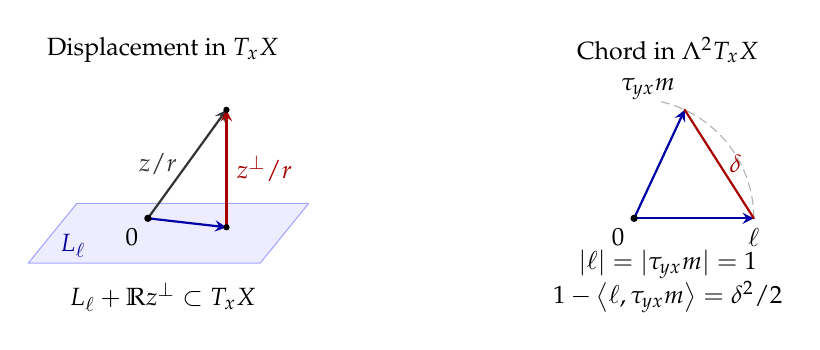
\begin{tikzpicture}[>=stealth, line cap=round, line join=round,
                    font=\small, scale=0.95]
  \begin{scope}
    \node at (0.2,2.25) {Displacement in \(T_xX\)};
    \filldraw[fill=blue!7, draw=blue!35]
      (-1.6,-0.6) -- (1.5,-0.6) -- (2.15,0.2) -- (-0.95,0.2) -- cycle;
    \node[blue!60!black] at (-1.0,-0.37) {\(L_\ell\)};
    \coordinate (O) at (0,0);
    \coordinate (Zt) at (1.05,-0.12);
    \coordinate (Z) at (1.05,1.45);
    \draw[->,thick,blue!65!black] (O) -- (Zt);
    \draw[->,thick,black!80] (O) -- (Z)
      node[midway,left] {\(z/r\)};
    \draw[->,thick,red!65!black] (Zt) -- (Z)
      node[midway,right] {\(z^\perp/r\)};
    \fill (O) circle (1.4pt);
    \node[below left] at (O) {\(0\)};
    \fill (Zt) circle (1.2pt);
    \fill (Z) circle (1.2pt);
    \node at (0.2,-1.05) {\(L_\ell+\R z^\perp\subset T_xX\)};
  \end{scope}
  \begin{scope}[xshift=6.5cm]
    \node at (0.45,2.25) {Chord in \(\Lambda^2T_xX\)};
    \coordinate (O) at (0,0);
    \coordinate (A) at (1.6,0);
    \coordinate (B) at (65:1.6);
    \draw[densely dashed,black!30] (1.6,0) arc (0:78:1.6);
    \draw[->,thick,blue!65!black] (O) -- (A);
    \draw[->,thick,blue!65!black] (O) -- (B);
    \draw[thick,red!65!black] (A) -- (B)
      node[midway,right] {\(\delta\)};
    \node[below] at (A) {\(\ell\)};
    \node[above left] at (B) {\(\tau_{yx}m\)};
    \fill (O) circle (1.4pt);
    \node[below left] at (O) {\(0\)};
    \node at (0.45,-0.62) {\(|\ell|=|\tau_{yx}m|=1\)};
    \node at (0.45,-1.05) {\(1-\ip{\ell}{\tau_{yx}m}=\delta^2/2\)};
  \end{scope}
\end{tikzpicture}
\caption{The two factors in the tangential cutoff estimate.
The left panel lies in the subspace spanned by \(L_\ell\) and
the normal displacement. The right panel lies in the span of
two unit bivectors, in a different ambient vector space.
Closedness produces the product \(\delta|z^\perp|/r\).
The squared integrals of its factors are \(\ang_r=O(r^4)\)
and \(\trans_r=o(r^2)\), respectively.}
\label{fig:cutoff-geometry}
\end{figure}

Fix \((x,\ell)\). Choose orthonormal normal coordinates
\(z=z_x(y)\) with \(\ell=e_1\wedge e_2\), and put
\(h_r(z)=h(|z|^2/r^2)\).
At the fixed center \(x\), first variation of squared
distance gives
\(d_x[d_g(x,y)^2](e_i)=-2z_i\). Hence, for \(i=1,2\),
\begin{equation}\label{eq:center-derivative}
df_r(x)e_i=-r^{-2}\int_X\partial_{z_i}h_r\dd\mu(y).
\end{equation}
This differentiates the scalar distance kernel. We now
freeze \(x,\ell\), and these coordinates, and use closedness
of \(T\) in the \(y\) variable.

Coordinate covectors in normal coordinates differ from
radially parallel covectors by \(O(|z|^2)\). Indeed, the
Jacobi equation along \(t\mapsto\exp_x(tz)\), in a parallel
frame, has curvature coefficient \(O(|z|^2)\). The field
with initial data \((0,v)\) is therefore
\(tv+O(|z|^2|v|)\) for \(0\le t\le1\), giving
\(\tau_{yx}\circ d(\exp_x)_z=\Id+O(|z|^2)\).
Inverting gives the same estimate for coordinate covectors.
Since both line bivectors have norm one,
\begin{equation}\label{eq:quadratic-coordinate}
(dz_1\wedge dz_2)(m)
=\ip{\ell}{\tau_{yx}m}+O(r^2)
=1-\tfrac12\delta^2+O(r^2)\qquad(|z|<r).
\end{equation}
All errors are uniform. Comparing
\eqref{eq:center-derivative} with the \(P\) part of the
current below, and bounding its \(Q\) part, gives
\begin{align}
\left|df_r(x)e_i+
r^{-2}T\bigl((\partial_{z_i}h_r)\,dz_1\wedge dz_2\bigr)\right|
&\le Cr^{-3}\int_{d_g(x,y)<r}(\delta^2+r^2)
                    \dd\lambda(y,m)\nonumber\\
&\quad+Cr^{-3}\int_{B_r(x)}|Q|\vol.
\label{eq:comparison-error}
\end{align}
After integration against \(\lambda(x,\ell)\), its first
term is \(O(r)\) by \eqref{eq:abstract-angular}. Its
\(r^2\) term is \(O(r)\) by \eqref{eq:abstract-growth}.
Its last term tends to zero by Fubini and
\eqref{eq:q-cutoff}. Thus the integrated comparison error
vanishes.

For \(i=1\), apply closure to \(d(h_rdz_2)\); for \(i=2\),
apply it to \(d(h_rdz_1)\). These one-forms are compactly
supported in the chart and extend smoothly by zero.
Since \(d(dz_j)=0\), each
\(T\bigl((\partial_{z_i}h_r)\,dz_1\wedge dz_2\bigr)\)
is, up to sign, a sum of terms
\[
T\bigl((\partial_{z_a}h_r)\,dz_a\wedge dz_j\bigr),
\qquad a=3,4,\quad j\in\{1,2\}.
\]
For the normal derivatives,
\[
|\partial_{z_a}h_r|
\le Cr^{-1}\left|\pr_{L_\ell^\perp}(z/r)\right|.
\]
The mixed coordinate two-forms satisfy
\[
|(dz_a\wedge dz_j)(m)|\le C(\delta+r^2).
\]
Indeed their radially parallel counterparts vanish on
\(\ell\), and their coordinate error is \(O(r^2)\).

The integrated \(Q\) and \(r^2\) errors are controlled as
in \eqref{eq:comparison-error}. Including the outer factor
\(r^{-2}\), the remaining term is at most
\[
Cr^{-3}\iint_{d_g(x,y)<r}
\delta\left|\pr_{L_\ell^\perp}(z_x(y)/r)\right|
\dd\lambda(y,m)\dd\lambda(x,\ell).
\]
By Cauchy--Schwarz, \eqref{eq:abstract-angular}, and
Lemma~\ref{lem:transverse}, this is bounded by
\begin{equation}\label{eq:critical-scaling}
Cr^{-3}\sqrt{\ang_r}\sqrt{\trans_r}
=r^{-3}O(r^2)o(r)=o(1).
\end{equation}
The second squared integral is exactly \(\trans_r\),
since its integrand does not depend on \(m\).
Combining with \eqref{eq:comparison-error} proves
\eqref{eq:tangential-cutoff}. No derivative of a
center-dependent frame occurs: first variation was
applied before the fixed-chart current tests.

\subsection*{Passing to the positive-density set}

Let \(b:\R\to\R\) be smooth with \(b(0)=0\).
On the uniformly bounded range of \(f_r\), both \(b\)
and \(b'\) are bounded. Dominated convergence gives
\begin{equation}\label{eq:weighted-current-limit}
b(f_r)T\longrightarrow b(c_h\theta)P
\end{equation}
as currents. For \(P\) this follows from pointwise
convergence of \(f_r\). For \(Q\) it follows from
\eqref{eq:theta-volume} and \(Q\in L^1\).

If \(\eta\) is a smooth one-form, closedness of \(T\)
and the product rule give
\[
(b(f_r)T)(d\eta)
=-T\bigl(b'(f_r)\,df_r\wedge\eta\bigr).
\]
The \(Q\) contribution tends to zero by
\eqref{eq:q-full-derivative}. A line bivector \(\ell\)
evaluates \(df_r\wedge\eta\) using only the restriction
of \(df_r\) to \(L_\ell\), so the \(P\) contribution
tends to zero by \eqref{eq:tangential-cutoff}.
It follows from \eqref{eq:weighted-current-limit} that
\(b(c_h\theta)P\) is closed.

Finally take \(b_n(s)=1-e^{-ns}\). On the relevant
nonnegative range, \(0\le b_n\le1\) and
\(b_n(c_h\theta)\to\ind_E\).
A second dominated-convergence limit proves that
\(P_E=\ind_EP\) is closed. The limits are successive:
first \(r\downarrow0\) for each fixed \(n\), then
\(n\to\infty\). No bound on \(b_n'\) uniform in \(n\)
is required.
\end{proof}

\section{The final pairing}\label{sec:conclusion}

\begin{proof}[Proof of Theorem~\ref{thm:main}]
Let \(\omega\) be a smooth closed form taming \(J\).
Suppose for contradiction that there is no compatible
symplectic form, and take \(P,Q,T,\lambda,\mu\) from
Proposition~\ref{prop:separation}. Propositions
\ref{prop:growth} and \ref{prop:energy} verify all the
hypotheses of Theorem~\ref{thm:splitting}.
Consequently the current \(P_E=\ind_{\{\theta>0\}}P\)
is closed. Set
\[
P'=\ind_{X\setminus E}P,\qquad
T'=P'+Q=T-P_E.
\]
Then \(T'\) is closed. The current \(P'\) is represented
by the restriction \(\lambda'\le\lambda\) to base points
outside \(E\), with projection
\(\mu'=\ind_{X\setminus E}\mu\).
We pair \(T\) with this residual current rather than with itself:
placing the second positive factor on zero-density centers makes
the previously bounded negative error in the pairing tend to zero.

We first show that the negative term in
\eqref{eq:positive-pairing} tends to zero for this
choice of \(P'\). For each \(y\notin E\),
\begin{equation}\label{eq:zero-density-tail}
r^{-2}\int_X(1+d_g(x,y)/r)^{-6}\dd\mu(x)
\longrightarrow0.
\end{equation}
On the inner ball and on every fixed dyadic shell this
follows from \(s^{-2}\mu(B_s(y))\to0\).
The quadratic mass bound dominates the shell contributions
by \(C2^{-4j}\), a summable sequence, giving the full
limit. The uniform bound \eqref{eq:shell} then permits
dominated convergence against \(\mu'\).
Discarding the nonnegative angular term in
\eqref{eq:positive-pairing} yields
\begin{equation}\label{eq:liminf}
\liminf_{r\downarrow0}\ip{S_rP}{*S_rP'}_{L^2}\ge0.
\end{equation}

Apply Lemma~\ref{lem:zero-pairing} to \(T'\).
Its regularizations are in \(L^2\), since \(P'\) has
measure coefficients and \(Q\in L^2\).
Expanding gives
\[
0=\ip{S_rP}{*S_rP'}
+\ip{S_rP}{*S_rQ}
+\ip{S_rQ}{*S_rP'}
+\|S_rQ\|_2^2.
\]
Both mixed terms tend to zero by
\eqref{eq:cross-vanish}, applied once to \(P\) and once
to \(P'\). Since \(S_rQ\to Q\) strongly in \(L^2\),
\eqref{eq:liminf} implies \(0\ge\|Q\|_2^2\).
Therefore \(Q=0\).

It follows that \(P=T\) annihilates all smooth closed
forms. In particular \(P(\omega)=0\). On the other
hand, \(\omega_x(\ell)>0\) on the compact bundle
\(\mathscr C\); it has a positive minimum there.
Equation~\eqref{eq:positive-representation} and
\(\lambda(\mathscr C)=1\) give \(P(\omega)>0\),
a contradiction.

The positive cone and the subspace of closed invariant
smooth forms therefore intersect. Any form in their
intersection is the required smooth compatible
symplectic form for \(J\).
\end{proof}

\section{The compatible cone}\label{sec:cones}

The distinction between existence and realization of a specified class
appears in the separating functional. For existence, it annihilates all
closed invariant forms. For a specified class, it need only annihilate
exact invariant forms. We first establish the estimates in this setting,
then identify the classes of the resulting currents.

\subsection{Invariant representatives and separation}

We retain the Hermitian metric, the projection \(R\), and the closed
lift \(B=dd^*G+H\) of Lemma~\ref{lem:lift}.
For a closed current \(D\), let
\(\mathfrak c(D)\in H^2(X;\R)\) denote its intersection-dual class:
\[
 D(\alpha)=\mathfrak c(D)\cdot[\alpha]
 \quad\text{for every smooth closed two-form }\alpha.
\]
Equivalently, \(\mathfrak c(D)\) is represented by the Hodge star of
the harmonic part of the distributional two-form associated with \(D\).

\begin{lemma}\label{lem:invariant-cohomology}
The classes represented by closed invariant forms are exactly
\(\mathcal V=(H_J^-)^\perp\). The intersection form is positive
definite on \(H_J^-\), and
\[
 H^2(X;\R)=\mathcal V\oplus H_J^-.
\]
The operator \(1-BR\) takes exact forms to exact invariant forms.
\end{lemma}

\begin{proof}
Closed anti-invariant forms are self-dual, hence harmonic. Their
intersection pairing is their \(L^2\) inner product, so it is positive
definite on their classes. Invariant and anti-invariant forms wedge to
zero pointwise.

For any closed two-form \(\alpha\), the form
\((1-BR)\alpha\) is closed and invariant, and
\[
 [\alpha]=[(1-BR)\alpha]+[HR\alpha],
\]
because \(BR\alpha=dd^*GR\alpha+HR\alpha\). The second summand
is represented by a closed anti-invariant form. The two subspaces are
orthogonal, and positive definiteness on the second makes their
intersection zero. This proves the decomposition and the assertion
about \(\mathcal V\).

If \(\alpha\) is exact, it is \(L^2\)-orthogonal to every harmonic
form. For a harmonic anti-invariant form \(\beta\),
\(\ip{R\alpha}{\beta}_{L^2}=\ip{\alpha}{\beta}_{L^2}=0\).
Thus \(HR\alpha=0\), and both \(BR\alpha\) and
\((1-BR)\alpha\) are exact.
\end{proof}

A current is called \emph{positive} here if it annihilates
anti-invariant forms and is nonnegative on pointwise semipositive
invariant forms. As in Proposition~\ref{prop:separation}, it has a
representation by a finite positive measure on \(\mathscr C\).
Its trace measure is the projection to \(X\).

\begin{lemma}[Prescribed-class separation]\label{lem:class-separation}
Let \(a\in\mathcal V\) have no compatible representative. There
are currents \(P,Q,T\in H^{-3}\), with \(P\) nonzero and positive,
such that
\begin{gather}
 P(F)=1,\qquad P\text{ annihilates exact invariant forms},
 \label{eq:class-exact-tests}\\
 T=P+Q\text{ is closed},\qquad RQ=Q=*Q,
 \label{eq:class-current}\\
 \mathfrak c(T)\in\mathcal V,\qquad
 \mathfrak c(T)\cdot a\le0.
 \label{eq:class-separator-sign}
\end{gather}
Moreover, a class \(b\in H^2(X;\R)\) is taming if and only if
\[
 b\cdot\mathfrak c(N)>0
 \quad\text{for every nonzero closed positive current }N.
\]
\end{lemma}

\begin{proof}
By Lemma~\ref{lem:invariant-cohomology}, the closed invariant
representatives of \(a\) form a nonempty affine space. Separate
this affine space from the open cone of positive invariant forms
in the Fr\'echet space of smooth invariant forms. Hahn--Banach
separation gives a nonzero continuous functional, nonnegative on
the positive cone and nonpositive on the affine space. It vanishes
on the direction space, which consists of exact invariant forms.
Indeed, translating by any real multiple of a direction preserves
the affine space, while positive scalings preserve the cone.
Extend the functional by \(1-R\) and normalize it as in
Proposition~\ref{prop:separation} to obtain \(P(F)=1\).
The same positivity argument gives its measure representation.

Define \(T(\alpha)=P((1-BR)\alpha)\) and
\(Q(\alpha)=-P(BR\alpha)\). Lemma~\ref{lem:invariant-cohomology}
shows that \(T\) annihilates every exact form, so it is closed.
The projection identities give \(RQ=Q=*Q\). A closed
anti-invariant form \(\beta\) lies in the kernel of the operator
used to construct \(G\); hence \(B\beta=\beta\) and
\(T(\beta)=0\). Thus \(\mathfrak c(T)\in\mathcal V\).
On a closed invariant representative of \(a\), the currents
\(T\) and \(P\) agree, proving \eqref{eq:class-separator-sign}.
The Sobolev assertion follows from the measure representation and
the order-zero lift, as in Proposition~\ref{prop:separation}.

For the last statement, a taming representative evaluates strictly
positively on every nonzero positive current. Conversely, if \(b\)
has no taming representative, separate its affine space of closed
representatives from the open cone of forms positive on complex
lines. The separator annihilates all exact forms. Since arbitrary
anti-invariant forms can be added to that cone, it also annihilates
all anti-invariant forms. It is therefore a nonzero closed positive
current \(N\), and \(b\cdot\mathfrak c(N)\le0\).
\end{proof}

\subsection{Pairings for currents of arbitrary class}

\begin{lemma}\label{lem:cohomological-pairing}
For closed currents \(D_1,D_2\in H^{-3}\),
\begin{equation}\label{eq:cohomological-pairing}
 \ip{S_rD_1}{*S_rD_2}_{L^2}
 =\mathfrak c(D_1)\cdot\mathfrak c(D_2).
\end{equation}
\end{lemma}

\begin{proof}
The forms \(*S_rD_i\) lie in \(H^3\), are distributionally closed,
and have the harmonic components representing \(\mathfrak c(D_i)\).
Here we use commutation with \(d^*,*\), and the fact that \(S_r\)
is the identity on harmonic forms. Their heat regularizations are
smooth closed representatives of these classes. The intersection
identity for smooth forms passes to the limit in \(L^2\).
In degree two on a four-manifold,
\(\alpha\wedge\beta=(*\alpha)\wedge(*\beta)\), giving
\eqref{eq:cohomological-pairing}.
\end{proof}

We record the estimates that apply to the separator in
Lemma~\ref{lem:class-separation}. In the next proposition, positive
currents are not required to have any prescribed cohomology class.

\begin{proposition}\label{prop:class-estimates}
Suppose that \(P\ne0\) is positive, annihilates exact invariant
forms, and \(T=P+Q\) is closed, where \(Q\in H^{-3}\) is
anti-invariant. Write \(\lambda\) for a positive measure representing
\(P\), and \(\mu\) for its trace. Then
\begin{gather}
 \mu(B_s(x))\le Cs^2,\qquad Q\in L^2,
 \label{eq:class-growth}\\
 \iint_{d_g(x,y)<r}|\ell-\tau_{yx}m|^2
       \dd\lambda(x,\ell)\dd\lambda(y,m)\le Cr^4.
 \label{eq:class-angular}
\end{gather}
Consequently the positive-density restriction \(P_E\) is closed,
where \(E=\{x:\lim_{s\downarrow0}s^{-2}\mu(B_s(x))>0\}\).

If \(A\) is any positive current whose trace has quadratic growth,
then
\begin{equation}\label{eq:class-mixed-limit}
 \lim_{r\downarrow0}\ip{S_rA}{*S_rQ}_{L^2}=0.
\end{equation}
Every closed positive current has quadratic trace growth.
\end{proposition}

\begin{proof}
Each radial test \(Du=(1-BR)dd_J^cu\) in
Section~\ref{sec:mass} is exact by
Lemma~\ref{lem:invariant-cohomology}. Its pointwise estimates
therefore give the quadratic growth bound under the present
annihilation hypothesis. The normalization \(P(F)=1\) is inessential:
for arbitrary finite mass it only changes the constant. In particular,
this argument applies to every closed positive current.

We will use the kernel estimates for any pair \(A_1,A_2\) of positive
currents with quadratic-growth trace measures \(\mu_1,\mu_2\).
Write \(\lambda_1,\lambda_2\) for their representing measures.
The proof of Lemma~\ref{lem:positive-pairing}, using
Lemma~\ref{lem:kernel} and \eqref{eq:angular-identity}, gives
\begin{align}
 \|S_rA_i\|_2&\le C_i r^{-1},\label{eq:general-smoothed-mass}\\
 \ip{S_rA_1}{*S_rA_2}_{L^2}
 &\ge cr^{-4}\iint_{d<r}|\ell-\tau_{yx}m|^2
            \dd\lambda_1(x,\ell)\dd\lambda_2(y,m)
 \nonumber\\
 &\quad-Cr^{-2}\iint(1+d/r)^{-6}
                     \dd\mu_1(x)\dd\mu_2(y),
 \label{eq:general-positive-pairing}
\end{align}
where \(d=d_g(x,y)\). These statements do not require either measure
to be dominated by the other. The shell bound
\eqref{eq:shell} holds separately for each \(\mu_i\), proving
the norm bound and a uniform bound on the negative term.

For any anti-invariant distribution \(W\) with \(S_rW\in L^2\),
Lemma~\ref{lem:mixing} and \eqref{eq:general-smoothed-mass} give
\begin{equation}\label{eq:general-mixed-bound}
 |\ip{S_rA_i}{*S_rW}_{L^2}|
 \le Cr\|S_rA_i\|_2\|S_rW\|_2
 \le C_i'\|S_rW\|_2.
\end{equation}
Apply \eqref{eq:cohomological-pairing} to \(T,T\).
Since \(Q\) is self-dual, expansion and these estimates yield
\[
 cr^{-4}\ang_r+\|S_rQ\|_2^2
 \le C+|\mathfrak c(T)^2|+C\|S_rQ\|_2,
\]
where \(\ang_r\) is the angular integral in
\eqref{eq:class-angular}. Hence \(S_rQ\) is uniformly bounded
in \(L^2\), and the angular bound follows. Weak compactness and
distributional convergence identify an \(L^2\) limit with \(Q\).

For smooth anti-invariant \(W\),
\[
 \ip{S_rA}{*S_rW}=A(S_r^2W)\longrightarrow A(W)=0.
\]
The uniform bound \eqref{eq:general-mixed-bound}, the \(L^2\)
contraction property of \(S_r\), and approximation by smooth
anti-invariant forms give \eqref{eq:class-mixed-limit}.
Finally, \eqref{eq:class-growth}--\eqref{eq:class-angular} verify
the hypotheses of Theorem~\ref{thm:splitting}, which proves that
\(P_E\) is closed.
\end{proof}

The next lemma permits pairing the zero-density part with positive
currents unrelated to the original separator.

\begin{lemma}[Residual pairings]\label{lem:general-residual}
Let \(A,P'\) be positive currents whose trace measures \(\nu,\mu'\)
have quadratic growth. Suppose
\[
 \lim_{s\downarrow0}s^{-2}\mu'(B_s(x))=0
 \quad\text{for }\mu'\text{-almost every }x.
\]
Then
\begin{equation}\label{eq:general-residual}
 \liminf_{r\downarrow0}\ip{S_rA}{*S_rP'}_{L^2}\ge0.
\end{equation}
\end{lemma}

\begin{proof}
We first show
\begin{equation}\label{eq:cross-small-density}
 (\mu'\times\nu)\{(x,y):d_g(x,y)<s\}=o(s^2).
\end{equation}
For small \(s\), choose an \(s\)-separated maximal set of centers
and let \(B_j\) be their radius-\(s\) balls. They cover \(X\),
and their fixed dilates have uniformly bounded overlap, by the
volume comparison in smooth coordinate charts. If \(x\in B_j\)
and \(d_g(x,y)<s\), then \(y\in2B_j\). Thus
\[
 (\mu'\times\nu)\{d<s\}
 \le\sum_j\mu'(B_j)\nu(2B_j).
\]
Bounded overlap gives
\[
 \sum_j\mu'(B_j)^2
 \le C\int_X\mu'(B_{2s}(x))\dd\mu'(x)=o(s^2).
\]
Indeed, the integrand divided by \(s^2\) is bounded by quadratic
growth and tends to zero at \(\mu'\)-almost every center.
Also
\[
 \sum_j\nu(2B_j)^2
 \le Cs^2\sum_j\nu(2B_j)=O(s^2).
\]
Cauchy--Schwarz proves \eqref{eq:cross-small-density}.

In \eqref{eq:general-positive-pairing}, discard the angular term.
The remaining negative error tends to zero: on \(d<r\), and on
each fixed shell \(2^jr\le d<2^{j+1}r\), this follows from
\eqref{eq:cross-small-density}. Quadratic growth bounds the shell
contributions by \(C2^{-4j}\), allowing summation by dominated
convergence. This proves \eqref{eq:general-residual}.
\end{proof}

\subsection{Proof of the cone description}

\begin{proof}[Proof of Theorem~\ref{thm:taming-cones}]
Adding a closed anti-invariant form does not change positivity on
complex lines. Lemma~\ref{lem:invariant-cohomology} therefore gives
\eqref{eq:tame-decomposition}. In particular \(\mathcal C\) is
nonempty. It is a convex cone of positive-square classes in
\(\mathcal V\), since its classes have closed taming representatives.

A compatible form wedges strictly positively with every taming form.
Indeed, in a unitary frame diagonalizing the compatible form, the
wedge product is a positive linear combination of the two positive
diagonal entries of the taming form's invariant part. Consequently
every \(a\in\mathcal K_J^c\) lies in \(\mathcal C\) and pairs
positively with every class in \(\mathcal C\), hence nonnegatively
with \(\overline{\mathcal C}\).

The compatible cone is open in \(\mathcal V\): add sufficiently
small linear combinations of closed invariant representatives of a
basis of \(\mathcal V\) to a compatible form. The intersection form
on \(\mathcal V\) is nondegenerate by
Lemma~\ref{lem:invariant-cohomology}. If \(a\cdot y=0\) for a
nonzero \(y\in\overline{\mathcal C}\), a sufficiently small
perturbation of \(a\) within the compatible cone would pair
negatively with \(y\). Thus every compatible class satisfies the
strict positivity in \eqref{eq:compatible-duality}.

Conversely, suppose \(a\in\mathcal C\) has this strict positivity
but no compatible representative. Apply
Lemma~\ref{lem:class-separation} and
Proposition~\ref{prop:class-estimates}. Let
\[
 P'=P-P_E,\qquad T'=P'+Q=T-P_E,\qquad
 y=\mathfrak c(T').
\]
Both \(P_E\) and \(T'\) are closed. Since \(P_E\) is invariant,
\(\mathfrak c(P_E)\in\mathcal V\), and hence \(y\in\mathcal V\).
The trace \(\mu'\) of \(P'\) satisfies the hypotheses of
Lemma~\ref{lem:general-residual}: it is bounded by \(\mu\) and
is concentrated where the latter has zero two-density.

We claim that \(y\in\overline{\mathcal C}\). Let \(N\) be any
nonzero closed positive current. Its trace has quadratic growth by
Proposition~\ref{prop:class-estimates}. By
\eqref{eq:cohomological-pairing},
\[
 y\cdot\mathfrak c(N)
 =\ip{S_rN}{*S_rP'}+\ip{S_rN}{*S_rQ}.
\]
The mixed term tends to zero by \eqref{eq:class-mixed-limit}, and
Lemma~\ref{lem:general-residual} bounds the lower limit of the first
term by zero. Thus \(y\cdot\mathfrak c(N)\ge0\). Since \(a\)
is taming, \((y+\eps a)\cdot\mathfrak c(N)>0\) for every
\(\eps>0\). The last part of Lemma~\ref{lem:class-separation}
shows that \(y+\eps a\) is taming. It also lies in \(\mathcal V\),
so \(y+\eps a\in\mathcal C\), proving the claim.

It follows that \(a\cdot y\ge0\), with strict inequality if
\(y\ne0\). If \(P'\ne0\), then \(y\ne0\). To see this,
suppose \(y=0\) and pair \(T'\) with itself using
\eqref{eq:cohomological-pairing}. We obtain
\[
 0=\ip{S_rP'}{*S_rP'}+2\ip{S_rP'}{*S_rQ}+\|S_rQ\|_2^2.
\]
The residual lemma, the mixed-term limit, and strong \(L^2\)
convergence of \(S_rQ\) force \(Q=0\). Then the nonzero positive
current \(P'=T'\) evaluates strictly positively on a closed tamer,
contrary to \(\mathfrak c(T')=0\).

Finally, a taming representative of \(a\) gives
\(a\cdot\mathfrak c(P_E)\ge0\), strictly if \(P_E\ne0\).
At least one of \(P_E,P'\) is nonzero. Therefore
\[
 a\cdot\mathfrak c(T)
 =a\cdot\mathfrak c(P_E)+a\cdot y>0,
\]
contradicting \eqref{eq:class-separator-sign}. This proves
\eqref{eq:compatible-duality}.
\end{proof}

\begin{proof}[Proof of Corollary~\ref{cor:taming-cones}]
The subspace \(H_J^-\) is positive definite, while its orthogonal
complement \(\mathcal V\) contains the nonempty positive-square
cone \(\mathcal C\). Hence \(h_J^-\le b_2^+-1\). If equality
holds, the intersection form on \(\mathcal V\) has signature
\((1,b_2^-)\). Convexity puts \(\mathcal C\) in one component
of its positive-square cone. Every element of that component pairs
strictly positively with every nonzero element of its closure,
by Cauchy--Schwarz in coordinates of signature
\((+,-,\ldots,-)\). Thus all \(a\in\mathcal C\) satisfy
\eqref{eq:compatible-duality}, and
\(\mathcal C=\mathcal K_J^c\). Equation
\eqref{eq:tame-decomposition} gives the asserted identity.
If \(b_2^+=1\), the inequality forces \(h_J^-=0\), proving the
last assertion.
\end{proof}

\begin{example}[Strict inclusion on the four-torus]\label{ex:strict-cones}
On \(X=\R^4/\mathbb Z^4\), use the Euclidean metric and standard
orientation, and put \(e^{ij}=dx_i\wedge dx_j\). Set
\[
 U=e^{12}+e^{34},\qquad V_0=e^{13}-e^{24},\qquad
 W=e^{14}+e^{23},
\]
\[
 f=\tfrac14\sin(2\pi x_1),\qquad
 k=\tfrac14\sin(2\pi x_2),\qquad
 r=(1+f^2+k^2)^{1/2}.
\]
The form \(F=(U+fV_0+kW)/r\) is self-dual and has squared norm
two, so it is the fundamental form of a smooth orthogonal almost
complex structure \(J\) of this orientation. The form
\[
 \eta=U+2f e^{13}+2k e^{23}
\]
is closed. Its self-dual part is \(rF\), so it is invariant, and
its anti-self-dual part is
\[
 f(e^{13}+e^{24})+k(e^{23}-e^{14}).
\]
Its Hermitian eigenvalues are \(r\pm\sqrt{f^2+k^2}>0\).
Thus \(\eta\) is compatible. The sine terms are exact, giving
\([\eta]=[U]\).

A closed anti-invariant form is self-dual and harmonic for the flat
metric, hence is a constant combination \(aU+bV_0+cW\).
Orthogonality to \(F\) gives \(a+bf+ck=0\) everywhere. Varying
\(x_1,x_2\) yields \(a=b=c=0\); thus \(H_J^-=0\).
The closed forms \(U\pm V_0\) have invariant projections
\((1\pm f)F/r\), so both tame \(J\). Their classes pair to zero,
since \(U^2=V_0^2\). Neither class can have a compatible
representative, which would wedge strictly positively with a tamer
in the other class. Hence
\[
 \mathcal K_J^c+H_J^-=\mathcal K_J^c
 \subsetneq\mathcal K_J^t.
\]
In Theorem~\ref{thm:taming-cones}, the class \([U+V_0]\) fails
the strict positivity test against \([U-V_0]\in\mathcal C\),
and conversely.
\end{example}

\begingroup
\small
\bibliographystyle{plain}
\bibliography{references}
\endgroup
\end{document}
